\chapter{Development}
In this section, we will describe the development process of the project. We will start by describing the usage of Eclipse Ditto and its integration with the Web Of Things, then we will describe some programming choices for the development of the project.

\section{Eclipse Ditto}
Ditto is an open-source technology for building simple digital twins that are mirroring some devices.
The technology potentially mirrors millions and billions of digital twins residing in the digital world with physical ``Things''.
This simplifies developing IoT solutions since there is no need to know how the physical ``Things'' are connected:
a thing can just be used as any other web service via its digital twin.


\section{Ditto's architecture}
Ditto consists of multiple ``microservices'' each of which is defined by:
\begin{itemize}
  \item its own data store which only this microservice may access and write to
  \item an API in form of signals (commands, command responses, events)
  \item can be accessed by other services only via the defined signals
\end{itemize}
All microservices can communicate asynchronously in a Ditto cluster (via Akka Remoting).

In figure\ref{fig:ditto-architecture} can be seen the architecture of Ditto and its components.

\begin{figure}[H]
  \centering
  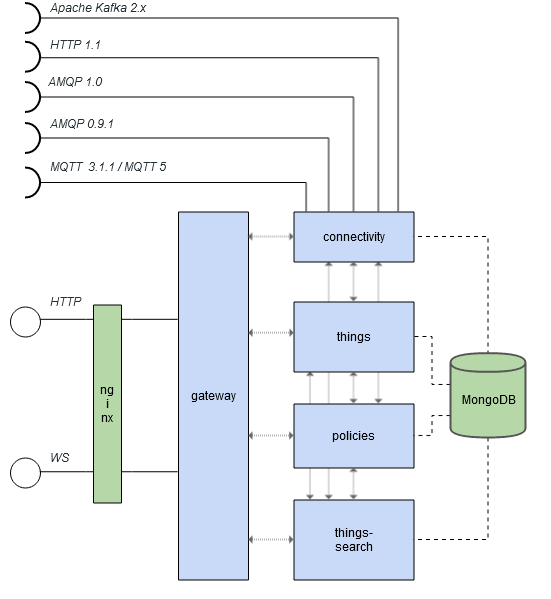
\includegraphics[width=0.7\textwidth]{img/ditto-architecture.png}
  \caption{Ditto architecture}
  \label{fig:ditto-architecture}
\end{figure}

The components of Ditto are:
\begin{itemize}
  \item Policies: manages persistence and enforcement (authorization) of Policies
  \item Things: manages persistence and enforcement (authorization) of Things and Features
  \item Things-Search: that tracks changes to Things, Features, Policies and updates an optimized search index. Also executes queries on this search index
  \item Gateway: that provides HTTP and WebSocket API
  \item Connectivity: that manages the persistence of Connections as well as sends Ditto Protocol messages to external message brokers and receives messages from them
\end{itemize}






\section{The Web of Things integration}
As with other platforms for digital twins (e.g. Microsoft Azure Digital Twins), Ditto is not dealing with interoperability and this is the main reason why is so important to have a semantic level.
In fact, this provides a common way to describe information and actions to interact with digital twins without knowing the technology used to model them.

Even though Ditto provides its own language to describe digital twins since version 2.4.0 (active by default with Ditto 3.0.0) they added support for W3C WoT (Web Of things) by referencing WoT Thing Model in Ditto managed twins for describing the Things' capabilities.
Using this integration, Ditto-managed digital twins can be linked to WoT ``Thing Models'' from which Ditto can create WoT ``Thing Descriptions'' containing the API descriptions of the twins.

As they declared in their website\footnote{\url{https://www.eclipse.org/ditto/2022-03-03-wot-integration.html}}, this integration takes a big step forward towards:
\begin{itemize}
    \item increased interoperability
    \item introspection of twins to find out their capabilities
    \item addition of semantic context to Ditto managed digital twins and their capabilities
    \item description of Ditto twin HTTP APIs in an open, established, well specified, ``web optimized'', active IoT standard
    \item backing Ditto managed twins with WoT models, also supporting ``brownfield'' setups, without the need for actual devices to be aware of WoT
    \item opening the door to a new ecosystem of tools
\end{itemize}

The idea of the thing description is that a device (or e.g. a digital twin service acting as intermediate) describes in a standardized way which capabilities in form of \textbf{properties}, \textbf{actions} and \textbf{events} a Thing provides and which input/output can be expected when interacting with it.
A TD contains the so-called \textbf{forms} for the mentioned interaction capabilities which map those rather abstract concepts to actual endpoints, e.g. to HTTP endpoints, HTTP verbs and HTTP headers etc. but also other protocol bindings e.g. MQTT or CoAP.

For this project, we exploited some of the benefits of this integration:
\begin{itemize}
    \item possibility to define a model for data (Ditto Thing attributes + Ditto Feature properties)
    \item possibility to define a model for messages
    \item capability to provide semantic context (using JSON-LD), e.g. by referencing existing ontologies
    \item Ditto-managed twins can describe themselves if backed by a WoT Thing Model; the twin can tell you (when asking for Accept: application/td+json content-type) exactly what it is capable of and which HTTP endpoints to invoke to access data / send messages
    \item utilization of the tooling landscape / open ecosystem evolving around the WoT standard, e.g.:
    the Eclipse edi{TD}or online editor for WoT TDs and TMs
\end{itemize}

In tables \ref{tab:ditto-wot-thing} and \ref{tab:ditto-wot-feature} we can see the mappings of the concepts between Ditto and WoT.

\begin{table}[H]
    \begin{tabular}{|p{0.3\textwidth}|p{0.6\textwidth}|}
    \hline
    \textbf{WoT element} & \textbf{Ditto concept} \\ \hline
    Thing & Ditto Thing\\ \hline
    Properties & Thing attributes\\ \hline
    Actions & Thing messages with Direction to (messages in the ``inbox'') of a Thing ID.\\ \hline
    Events & 	Thing messages with Direction from (messages in the ``outbox'') of a Thing ID.\\ \hline
    Composition via tm:submodule & Thing features representing different aspects of a Ditto Thing.\\ \hline
    \end{tabular}
    \caption{Mapping between Ditto and WoT for the ``Thing'' level}
    \label{tab:ditto-wot-thing}
\end{table}

\begin{table}[H]
    \begin{tabular}{|p{0.3\textwidth}|p{0.6\textwidth}|}
    \hline
    \textbf{WoT element} & \textbf{Ditto concept} \\ \hline
    Thing & Feature. In Ditto, a Feature is an aspect of a Ditto Thing. As the Feature is defined by its properties and messages it supports, it maps to a WoT Thing. \\ \hline
    Properties & Feature properties \\ \hline
    Actions &	Feature messages with Direction to (messages in the ``inbox'') of a Thing ID + Feature ID combination. \\ \hline
    Events &	Feature messages with Direction from (messages in the ``outbox'') of a Thing ID + Feature ID combination. \\ \hline
    \end{tabular}
    \caption{Mapping between Ditto and WoT for the ``Feature'' level}
    \label{tab:ditto-wot-feature}
\end{table}

\section{Handlers implementation}
The code base of the project is written in \textit{Scala 3} using a monadic approach.

In fact, all domain actions take advantage of a monadic encoding of side effects, ranging from failure with an exception, to emitting events, to reading an immutable global state.
The same approach was applied to the handler's implementation for the domain events.

An example of such handlers can be found below.

\begin{lstlisting}[language=Scala]
  def handlePackagingMachineFailureEvent[M[_]: Monad: LiftIO: CanRaise[String]](
      event: PackagingMachineFailedDTO,
  ): M[Unit] =
    for
      r <- validate(event)
      message = managePackagingMachineFailure(PackagingMachineFailure(LocalTime.now(), r.batchID, r.cutterTemperature))
      _ <- IO.println("Sending an e-mail to the admin...").liftIO[M]
      _ <- sendEmail(message)
    yield ()
\end{lstlisting}

Implemented in the \texttt{Alerts} bounded context, the code of the handler of the Packaging Machine Failure event, validates the incoming event, converting the concept coming from another bounded context into a domain concept, then it calls the domain action \texttt{managePackagingMachineFailure} which will properly manage the failure and finally sends an email to the maintenance team with the resulting content of the action.

Another code example of a handler can be found in the \texttt{Maintenance} bounded context.
This represents the storage of the failure event in the database:

\begin{lstlisting}[language=Scala]
def packagingMachineFailureHandler[M[_]: Monad: LiftIO: CanRaise[String]](
    failure: PackagingMachineFailureDTO,
): M[Unit] =
  for
    failureEvent <- validate(failure)
    _ <- collectMachineFailure(failureEvent)
    _ <- writeFailureToDB(failureEvent)
  yield ()
\end{lstlisting}

\section{DTOs implementation}
All events are represented with external entities that need to be transformed into domain entities.
This was done by implementing a set of DTOs (Data Transfer Objects) for each event, which is used to validate the incoming events and transform them into domain entities.

A code example of the Packaging Machine Failure DTO:

\begin{lstlisting}[language=Scala]
final case class PackagingMachineMaintenanceDTO(maintenance: String)
object PackagingMachineMaintenanceDTO:
  given DTO[PackagingMachineFailure, PackagingMachineFailureDTO] = productTypeDTO

\end{lstlisting}

\section{REST API}
We exploited Ditto's sandbox for our digital twins and this comes with a well-documented REST API.
This allowed us to interact with the digital twins in a standard way enhancing the interoperability between different systems.
This is one of the most important features that Ditto provides since, other than the fact that it is a standard for client-side applications, it is also easy to use from the side of the industrial machine.
This is a difference from other solutions for digital twins like, for instance, Microsoft Azure Digital Twins, which instead provides SDKs for a limited number of programming languages.
